% Chapter 9

\chapter{Event Selection} % Chapter title
\label{ch:eventsel} 

The goal of this analysis is to identify events resembling \autoref{fig:simpmodel} in collisions in the \ac{ATLAS} detector. In order to do this, a \acf{SR} is defined with the goal of maximizing the identification efficiency of signal events while minimizing \ac{SM} backgrounds. However, because this analysis re-investigates an excess of events seen in Run 1 with the \ac{ATLAS} detector, the signal region was frozen and could not be re-optimized for the new, higher energy data in Run 2. 

The \ac{SR}, called SRZ, was predetermined, including events with two opposite-sign, same-flavor leptons that reconstruct a mass, \mll, close to that of the $Z$ boson, with the additional requirement of two jets, \met > 225 \gev, and \HT of at least 600 \gev. Additionally, a cut on $\Delta\phi(\text{jet}_{12},{\boldsymbol p}_{\mathrm{T}}^{\mathrm{miss}})$ was made in order to suppress \dyjets background events with mismeasured jets. In events where jet mismeasurement produces large amounts of \met, the ${\boldsymbol p}_{\mathrm{T}}^{\mathrm{miss}}$ vector should either align or anti-align with the mismeasured jet's trajectory based on whether its energy has been overestimated or underestimated. This cut vetoes events in which the two vectors are aligned, reducing the number of of events that will be included in the \ac{SR} due to the underestimation of jet energy. Though it would be possible to also veto events in which the vectors are anti-aligned, similar topologies can also be produced by signal processes, so no such requirement is made. 

Each of these \ac{SR} requirements was designed to minimize \ac{SM} backgrounds while keeping a high efficiency for potential signals. In the simplified models studied, for example, the number of jets is nearly always above two, as shown in \autoref{fig:sig_njets}, while \ac{SM} production peaks at zero jets. The same is true for \met and \HT, also depicted in \autoref{fig:sig_njets}; signal models result in events with high values for these quantities, while \ac{SM} processes are most likely to produce events with very little \met or \HT. For comparison, \autoref{fig:datamc_inc} shows these quantities for the \ac{SM} backgrounds in a region with at least two jets. The jet requirement slightly shapes the \HT spectrum, causing it to peak at about 100 \gev~rather than at zero.

\begin{figure}[!htb]
\centering
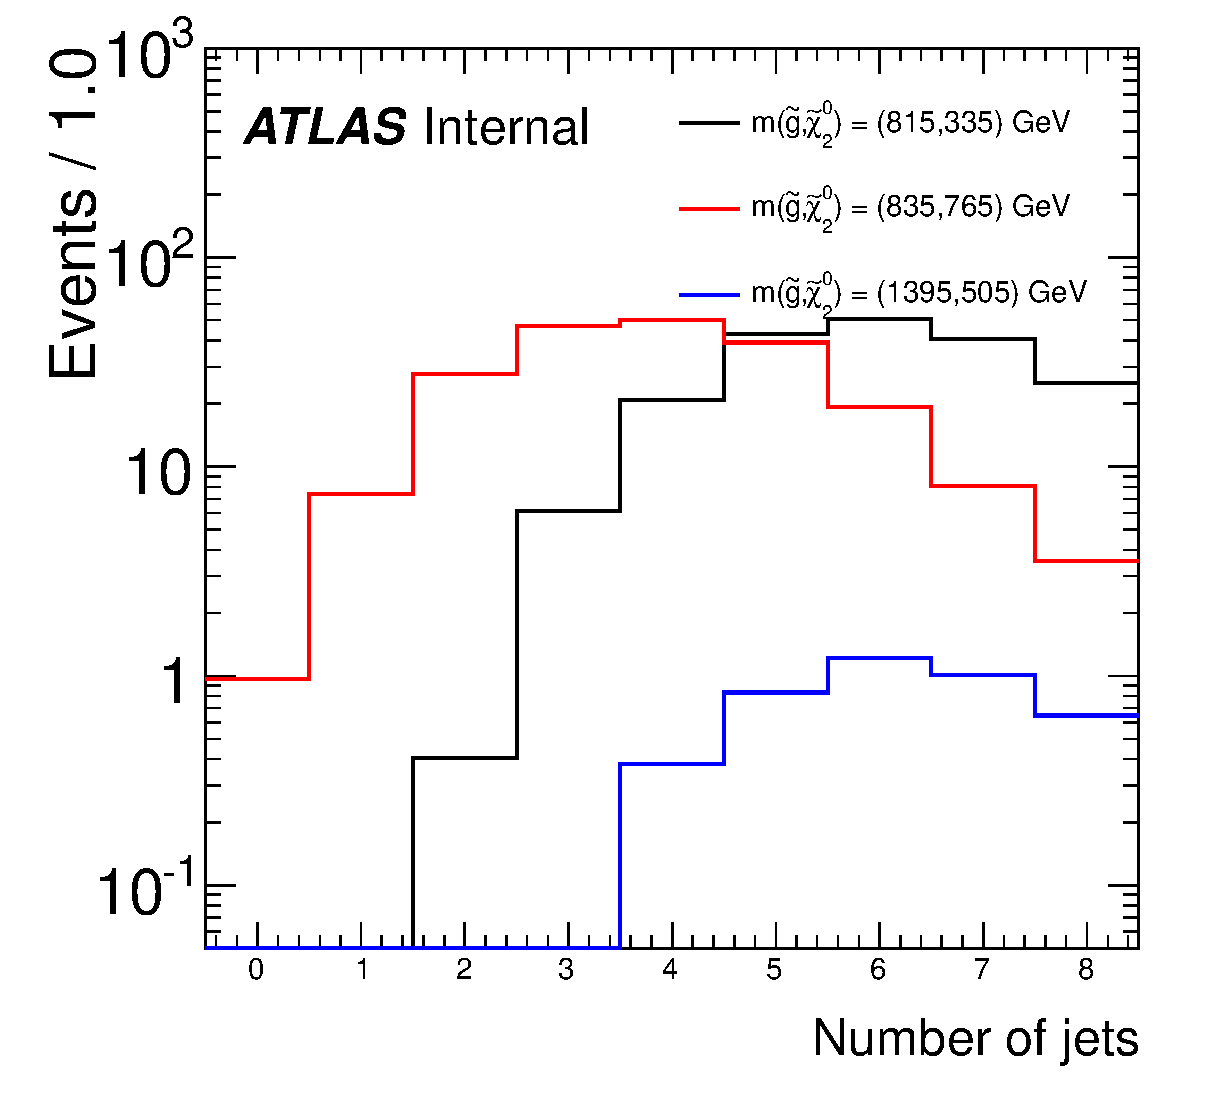
\includegraphics[width=.48\textwidth]{figures/signalacceptcontam/njets_R.eps}\\
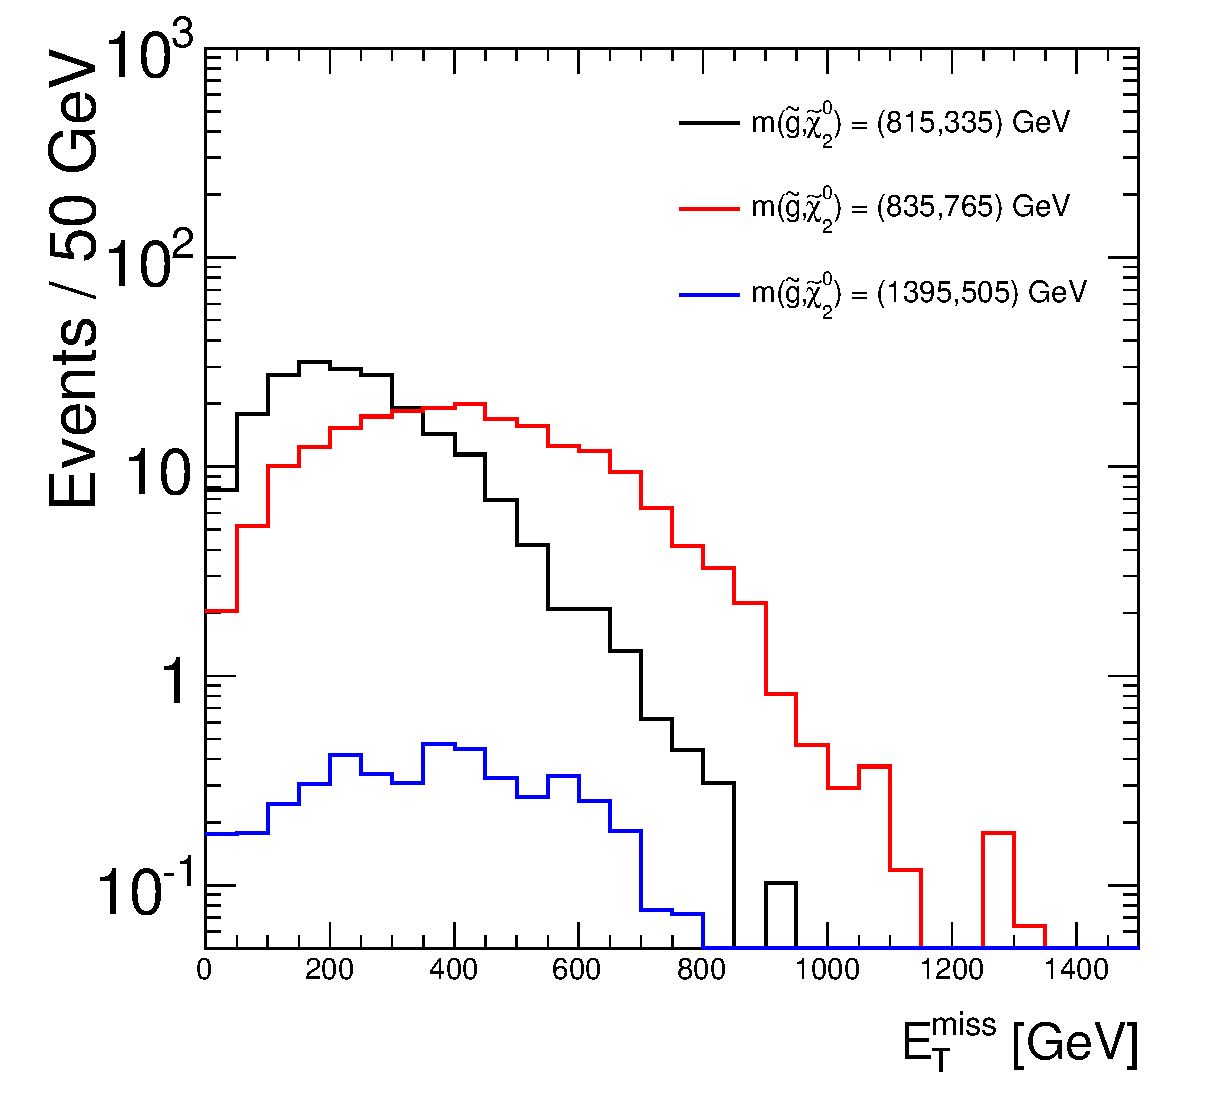
\includegraphics[width=.48\textwidth]{figures/signalacceptcontam/met_R.eps}
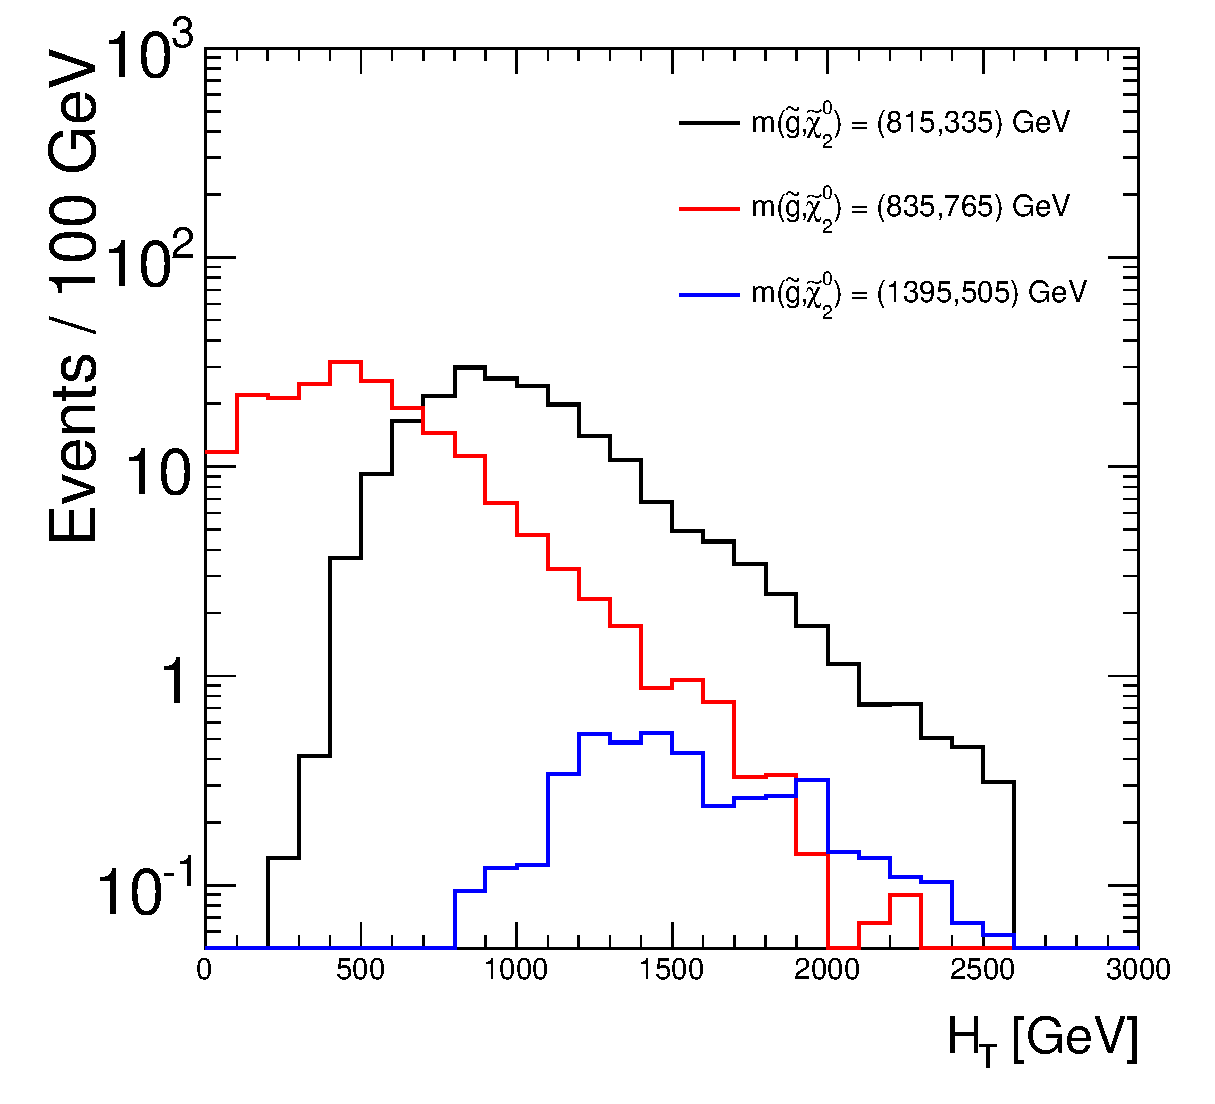
\includegraphics[width=.48\textwidth]{figures/signalacceptcontam/ht_R.eps}\\
\caption{
Number of jets (top), \HT (bottom left), and \met (bottom right) in three signal points, with $m(\go)$ = 815, 835, and 1395 \gev. 
\label{fig:sig_njets}
}
\end{figure}

\begin{figure}[!htb]
\centering
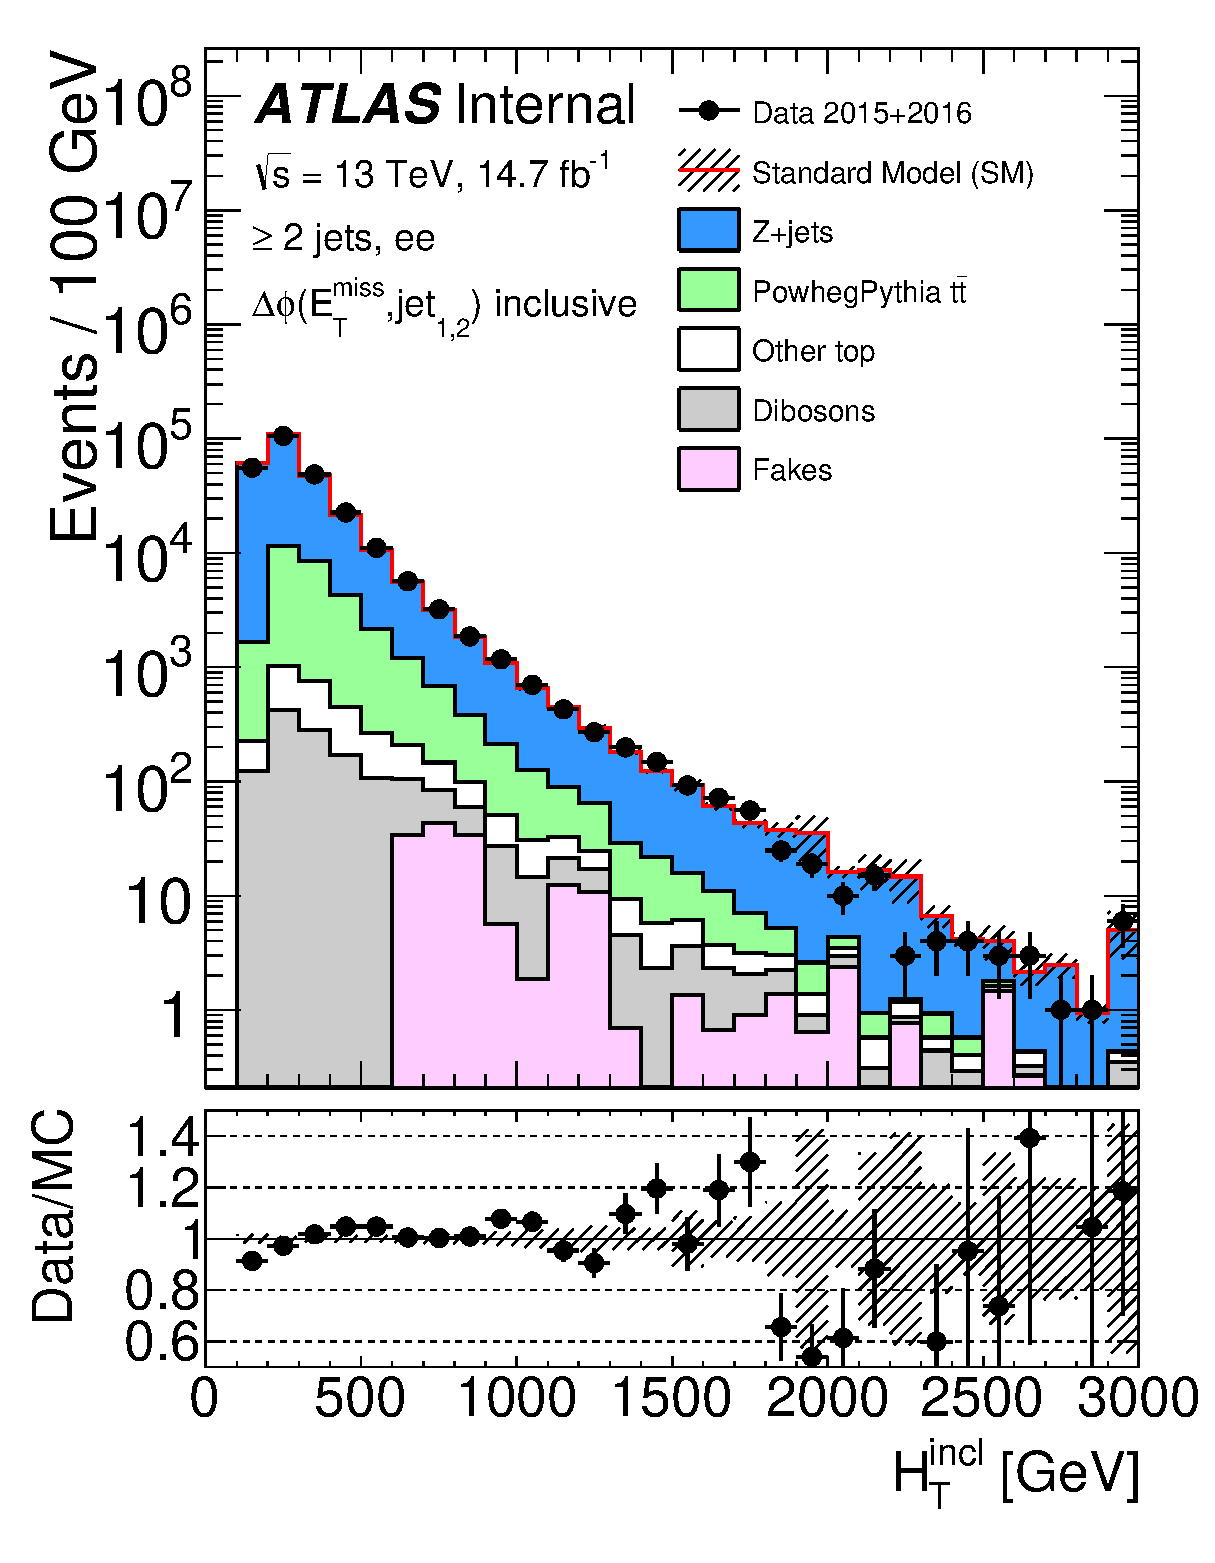
\includegraphics[width=.48\textwidth]{figures/signalacceptcontam/htincl_ee_preselection_R_a.eps}
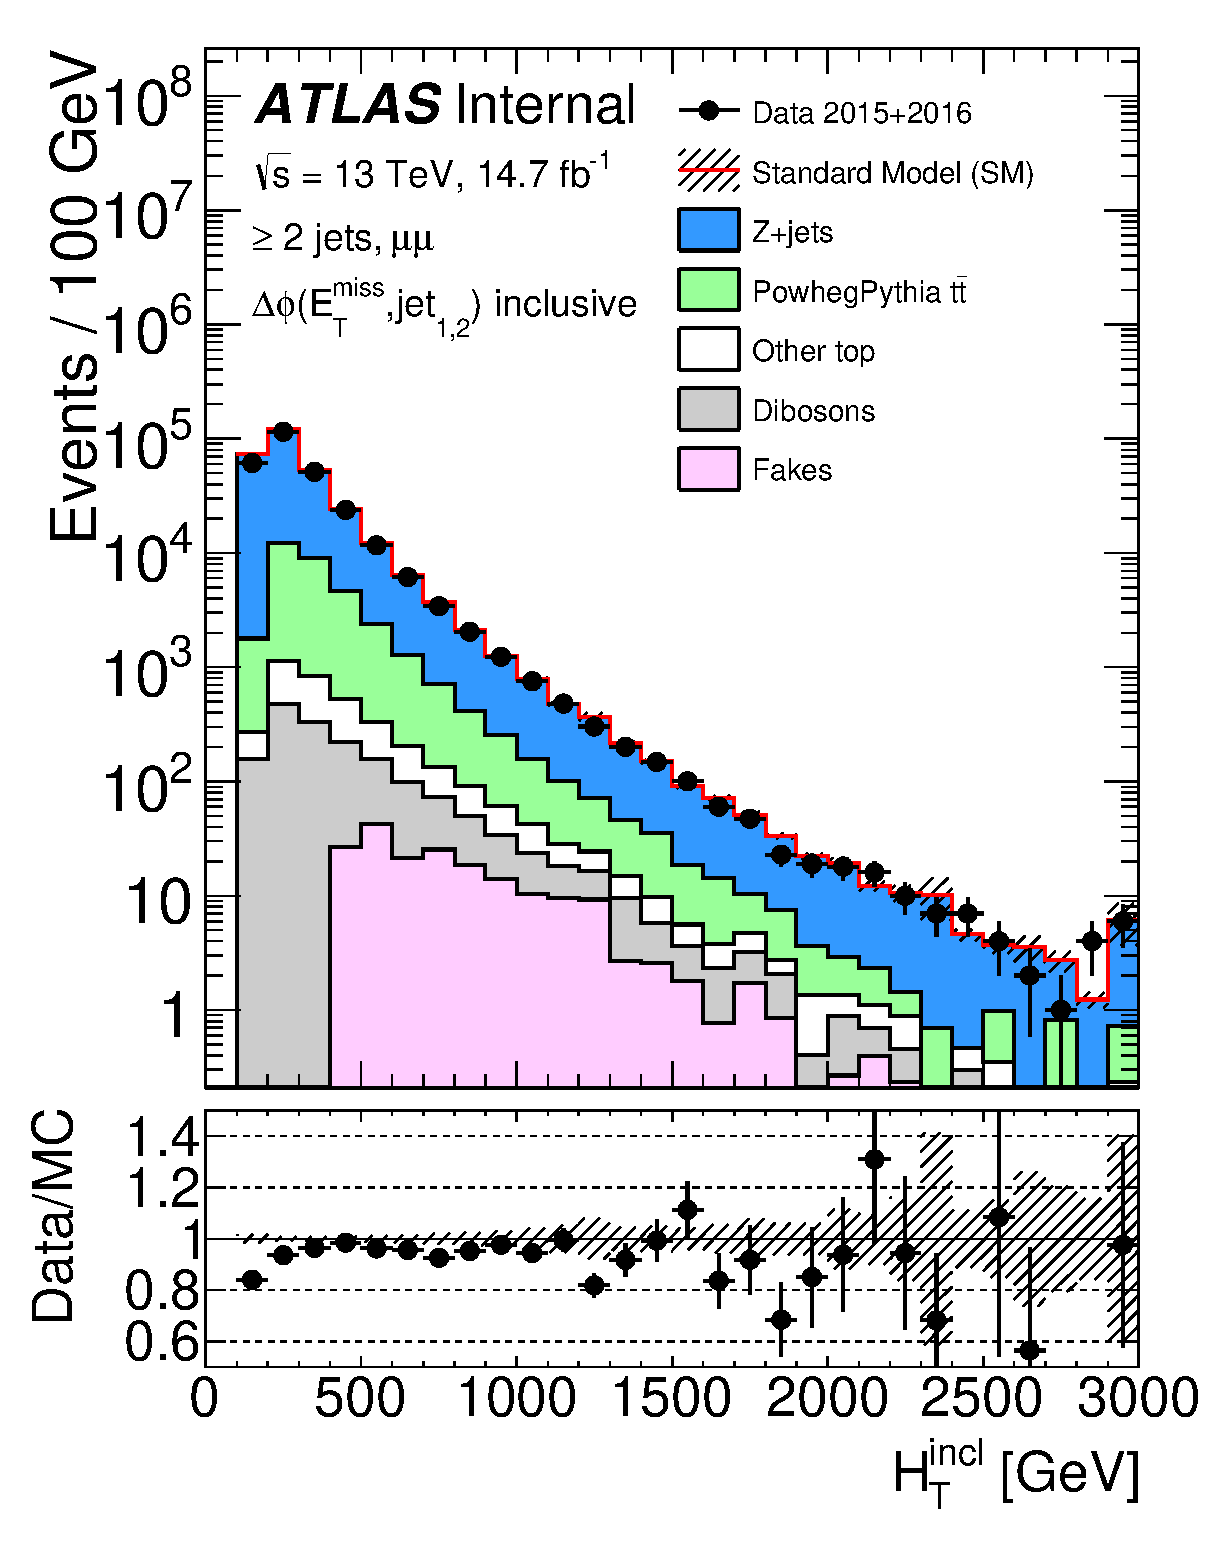
\includegraphics[width=.48\textwidth]{figures/signalacceptcontam/htincl_mm_preselection_R_a.eps}\\
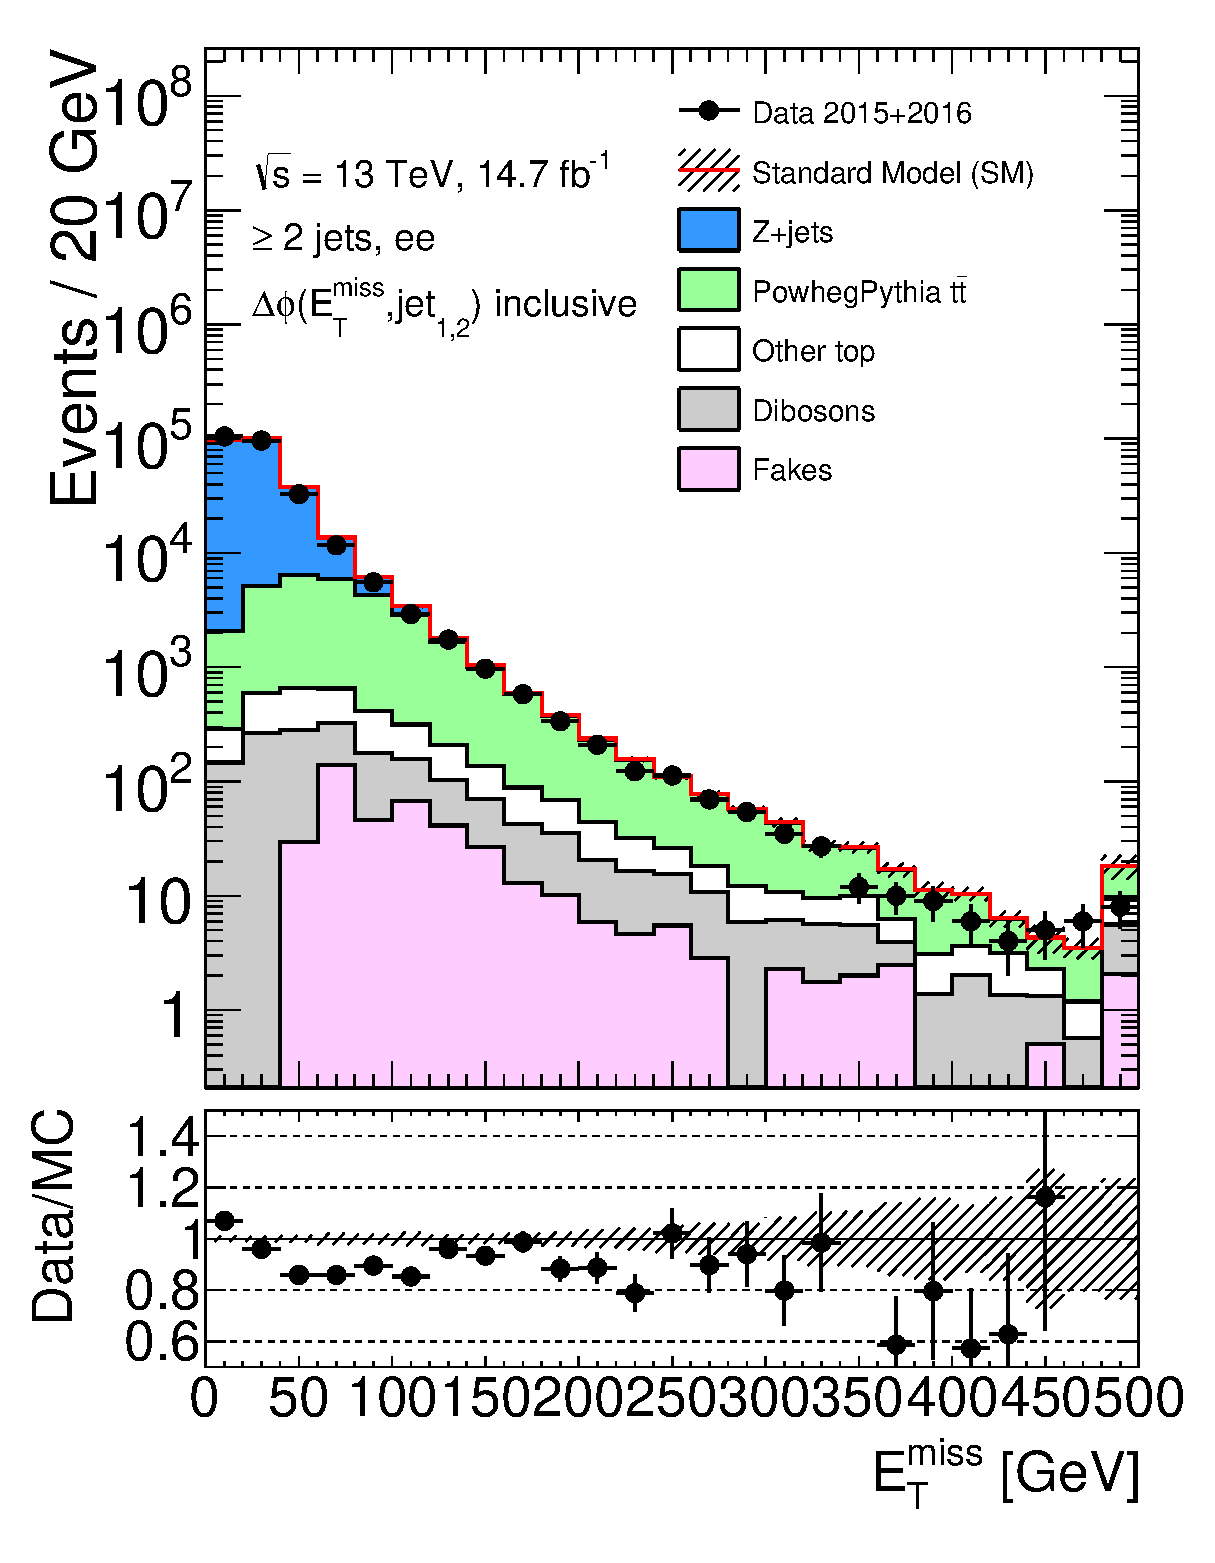
\includegraphics[width=.48\textwidth]{figures/signalacceptcontam/met_ee_preselection_R_a.eps}
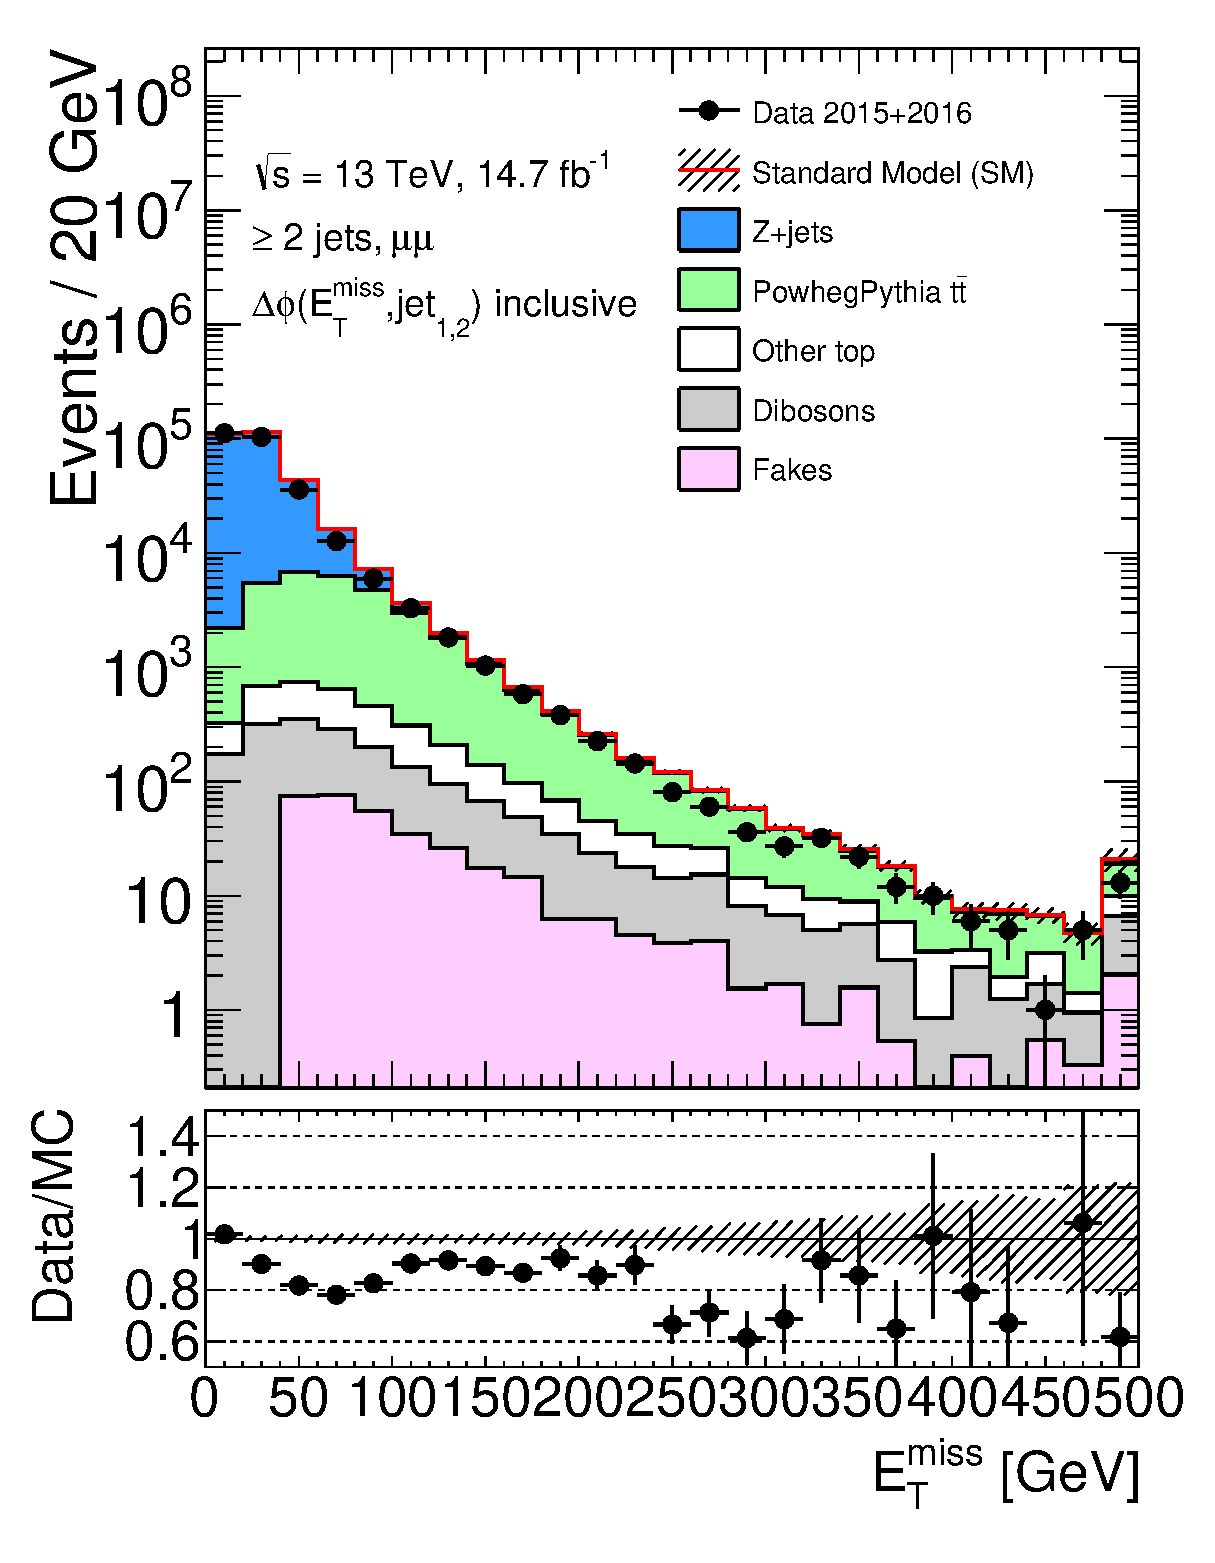
\includegraphics[width=.48\textwidth]{figures/signalacceptcontam/met_mm_preselection_R_a.eps}\\
\caption{
Comparison of data and \ac{MC} in an inclusive selection of events with at least two jets. Top is the \HT for these events, and \met is shown on the bottom. On the left is the $ee$ channel and on the right is the $\mu\mu$ channel. 
\label{fig:datamc_inc}
}
\end{figure}

The freezing of the \ac{SR} prevented re-optimization of the cuts for maximum sensitivity to a signal, but the search was still expected to be more sensitive than the previous iteration performed on 8 \tev~data. This is because the cross-section for production of this high-mass signal increased dramatically with the increased \ac{LHC} energy, while the cross-section for \ac{SM} processes increased at lower rates. With 20.3 fb$^{-1}$ of 8 \tev~data, the previous search had an expected exclusion on gluino masses up to about 950 \gev~\cite{SUSY-2014-10}, while with 14.7 fb$^{-1}$ of 13 \tev~data, this search has an expected exclusion on gluino masses up to about 1300 \gev~\footnote{The expected exclusions, discussed further in \autoref{ch:interpretations}, are made assuming the data exactly matches background predictions. The previous search had an observed exclusion on gluino masses up to about 850 \gev, which was lower than the expected exclusion due to the excess observed.}.

Though this \ac{SR} was fixed, the methods used to estimate the expected \ac{SM} backgrounds were not. A set of \acfp{CR} and \acfp{VR} were chosen to make these estimations possible. \acp{CR} are regions in which the collected data can be used to make an estimate of a \ac{SM} background in the \ac{SR}, while \acp{VR} are used to confirm that the background estimate based on the \ac{CR} is valid. Both \acp{CR} and \acp{VR} are designed to minimize contamination from the \ac{BSM} process being searched for. This is desirable because signal contamination in a \ac{CR} can lead to an overestimate of the \ac{SM} background in the \ac{SR}, disguising a genuine signal as background. Contamination in a \ac{VR}, where background estimates are being validated, can make it appear that the \ac{SM} background is not well described by an estimate, causing analyzers to adjust the method to account for the difference, and again, disguising the effect of the same signal in the \ac{SR}. 

The strategy for estimating the \ac{FS} background, for example, depends on a series of \acp{CR} and \acp{VR} depicted in \autoref{fig:region_diagrams}. One estimate, the flavor symmetry method, takes data from CR-FS, a different-flavor region with slightly wider \mll~bounds than the \ac{SR}, and uses these events to predict the contribution of flavor symmetric processes to SRZ. An independent method called a sideband fit uses a control region CRT to measure the flavor symmetric events outside of the $Z$ mass window, and uses \ac{MC} to extrapolate inside the $Z$ mass window to SRZ. In addition, both methods are validated at lower \met with an otherwise identical series of regions, with VRS corresponding to SRZ, VRT corresponding to CRT, and VR-FS corresponding to CR-FS. 

\begin{figure}[h]
\centering
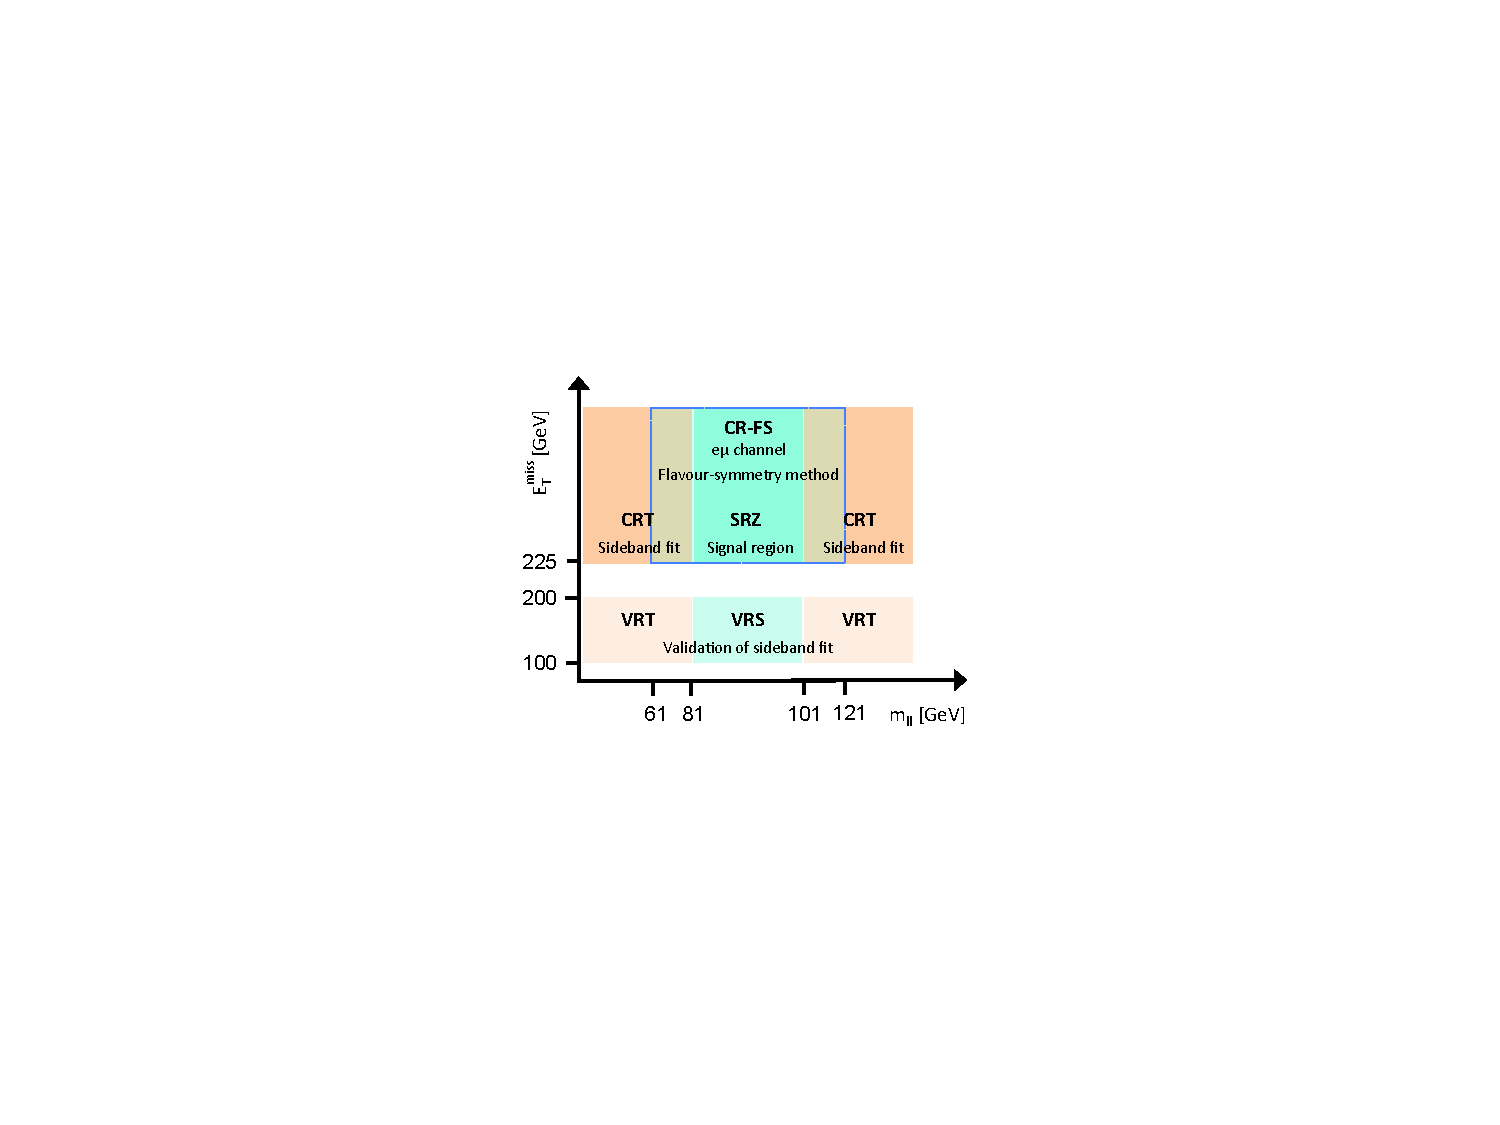
\includegraphics[width=.8\textwidth]{figures/fs/FSdiagram_v2.pdf}\\
\caption{
Schematic layout of the signal region, as well as the control and validation regions used to predict the \ac{FS} background. The regions displayed differ only by their \mll~and \met values, except for CR-FS, which contains different-flavor leptons, while all other regions contain same-flavor leptons \cite{this_paper}. 
\label{fig:region_diagrams}
}
\end{figure}

The background estimation methods, described in \autoref{ch:backgrounds}, each require their own set of these regions. The full list of regions used in this analysis can be seen in \autoref{tab:regions-z}. In addition to the \ac{FS} regions described above, there is one more \ac{CR}, CR-$\gamma$, which is a photon region used to predict the number of \dyjets events, a process described in \autoref{sec:bg-z}. Additional \acp{VR}, VR-ZZ, VR-WZ, and VR-3L, are introduced in order to validate the diboson and rare top backgrounds that are taken directly from \ac{MC}. There are several additional regions used in the estimation of the fakes and \dyjets contributions to the \ac{SR} that are defined in their respective sections. 

\begin{table}[htbp]
\begin{center}
\resizebox{\textwidth}{!}{
 \begin{tabular}{lcccccccc} %{\textwidth}{@{\extracolsep{\fill}}lcccccccc}
   \noalign{\smallskip}\hline\noalign{\smallskip}
     {\bf On-shell $Z$} &  {\bf \met}   &  {\bf $\HT$}  &  {\bf $n_{\text{jets}}$}  & {\bf $m_{\ell\ell} $}  &  {\bf SF/DF}  &  {\bf $\Delta\phi(\text{jet}_{12},{\boldsymbol p}\
_{\mathrm{T}}^\mathrm{miss})$ }  &  $m_{\text{T}}(\ell_{3},\met)$ &  $n_{\text{b-jets}}$ \\
     {\bf regions}       &  {\bf [\GeV]} &  {\bf [\GeV]} &                           &    {\bf [\GeV]}        &               &                                             &  [\GeV\
]                        &   \\
   \noalign{\smallskip}\hline\noalign{\smallskip}
   \multicolumn{2}{l}{Signal region} &&&&&& \\
   \noalign{\smallskip}\hline\noalign{\smallskip}
   SRZ  &  $> 225$  &  $> 600$  &  $\geq 2$  & $81 < m_{\ell\ell} < 101$  &  SF  &  $>0.4$ & $-$& $-$\\
   \noalign{\smallskip}\hline\noalign{\smallskip}
   \multicolumn{2}{l}{Control regions} &&&&&&  &  \\
   \noalign{\smallskip}\hline\noalign{\smallskip}
   CRZ              &  $\mathbf{< 60}$   &  $> 600$  &  $\geq 2$   &  $81 < m_{\ell\ell} < 101$       &  SF  & $>0.4$ & $-$  &  $-$ \\
   CR-FS            &  $> 225$  &  $> 600$  &  $\geq 2$   &  $\mathbf{61 < m_{\ell\ell} < 121}$       &  {\bf DF}  & $>0.4$ & $-$  &  $-$ \\
   CRT              &  $> 225$  &  $> 600$  &  $\geq 2$   &  $\mathbf{>40}$, $\mathbf{m_{\ell\ell} \notin [81,101]}$  &  SF  & $>0.4$ & $-$  &  $-$ \\
   CR$\gamma$       &  $-$        &  $> 600$  &  $\geq 2$   &  $-$                                                        &  {\bf $0\ell$, $1\gamma$}  & $-$ & $-$  &  $-$ \\
   \noalign{\smallskip}\hline\noalign{\smallskip}
   \multicolumn{2}{l}{Validation regions} &&&&&& \\
   \noalign{\smallskip}\hline\noalign{\smallskip}
   VRZ  &   $\mathbf{<225}$      &  $> 600$   &  $\geq 2$  &    $81 < m_{\ell\ell} < 101$       &  SF        & $>0.4$  & $-$ & $-$ \\
   VRT  &  {\bf 100--200}     &  $> 600 $  &  $\geq 2$  &    $\mathbf{>40}$, $\mathbf{m_{\ell\ell} \notin [81,101]}$  &  SF        & $>0.4$  & $-$ & $-$ \\
   VRS  &  {\bf 100--200}     &  $> 600 $  &  $\geq 2$  &    $81 < m_{\ell\ell} < 101$       &  SF        & $>0.4$  & $-$ & $-$ \\
   VR-FS & {\bf 100--200}     &  $> 600 $  &  $\geq 2$  &    $\mathbf{61 < m_{\ell\ell} < 121}$  &  {\bf DF}        & $>0.4$  & $-$ & $-$ \\
   VR-WZ  &  {\bf 100--200}   &     $-$      &   $-$        &         $-$                          &  $\mathbf{3\ell}$   &    $-$    & $<100$  &  $0$  \\
   VR-ZZ  &  {\bf $<100$}     &     $-$      &   $-$        &         $-$                          &  $\mathbf{4\ell}$   &    $-$    &  $-$      & $0$   \\
   VR-3L  &  {\bf 60--100}    &  $\mathbf{> 200}$  &  $\geq 2$  &   $81 < m_{\ell\ell} < 101$        &  $\mathbf{3\ell}$   & $>0.4$  & $-$ & $-$ \\
   \noalign{\smallskip}\hline\noalign{\smallskip}
\end{tabular}
} % end of resizebox
 \caption{Overview of all signal, control and validation regions used in the on-shell $Z$ search.
 More details are given in the text.
 %The \met~significance and soft-term fraction $f_{\text{ST}}$ needed in the seed regions for the jet smearing method
 %are defined in Sect.~\ref{sec:zjets}.
 The flavour combination of the dilepton pair is denoted as either \textit{SF} for same-flavor or \textit{DF} for different flavor.
 All regions require at least two leptons, unless otherwise indicated.
 In the case of CR$\gamma$, VR-WZ, VR-ZZ, and VR-3L the number of leptons, rather than a specific flavor configuration, is indicated.
The main requirements that distinguish the control and validation regions from the signal region are indicated in bold.
Most of the kinematic quantities used to define these regions are discussed in the text. The quantity $m_{\text{T}}(\ell_{3},\met)$
indicates the transverse mass formed by the \met and the lepton which is not assigned to either of the $Z$-decay leptons. }
\label{tab:regions-z}
\end{center}
\end{table}

\section{Trigger Strategy}
\label{sec:trig_strategy}

In order to collect data for the analysis, triggers must be chosen that provide good efficiency in each of the \ac{SR}, \ac{VR}, and \acp{CR}. This analysis primarily depends on triggers on leptons, which are required in nearly every region. To simplify the application of trigger scale factors, which correct \ac{MC} yields for a given trigger to match the data efficiencies, events are broken down into a series of kinematic ranges, each with a designated trigger. These regions can be seen in \autoref{tab:trigger_strat}.

\begin{table}[hbt]
\begin{center}
\resizebox{1\textwidth}{!}{
\begin{tabular}{l|cc}
\hline
 %& \hspace*{30mm} \\[-3mm]
Lepton \pt    & Trigger in 2015 & Trigger in 2016    \\
\hline\hline
\multicolumn{3}{l}{Di-electron channel} \\
\hline
$\pt(e_1) > 65$~\GeV                               & \texttt{HLT\_e60\_lhmedium} & \texttt{HLT\_e60\_lhmedium\_nod0} \\
$\pt(e_1) \leq 65$~\GeV                            & \texttt{HLT\_2e17\_lhloose} & \texttt{HLT\_2e17\_lhvloose\_nod0} \\
\hline
\multicolumn{3}{l}{Di-muon channel} \\
\hline
$\pt(\mu_1) > 52.5$~\GeV                             & \texttt{HLT\_mu50}          & \texttt{HLT\_mu50} \\
$\pt(\mu_1) \leq 52.5$~\GeV                          & \texttt{HLT\_mu24\_mu8noL1} & \texttt{HLT\_2mu14\_nomucomb} \\
\hline
\multicolumn{3}{l}{Electron-muon channel} \\
\hline
$\pt(e) > 65$~\GeV                                 & \texttt{HLT\_e60\_lhmedium} & \texttt{HLT\_e60\_lhmedium\_nod0} \\
$\pt(e) \leq 65$~\GeV~and $\pt(\mu) > 52.5$~\GeV     & \texttt{HLT\_mu50}          & \texttt{HLT\_mu50} \\
$\pt(e) \leq 65$~\GeV~and $\pt(\mu) \leq 52.5$~\GeV  & \multirow{2}{*}{\texttt{HLT\_e7\_lhmedium\_mu24}} & \multirow{2}{*}{\texttt{HLT\_e7\_lhmedium\_nod0\_mu24}} \\
\hspace*{5mm} and $\pt(e) < \pt(\mu)$ & \\
$\pt(e) \leq 65$~\GeV~and $\pt(\mu) \leq 52.5$~\GeV  & \multirow{2}{*}{\texttt{HLT\_e17\_lhloose\_mu14}} & \multirow{2}{*}{\texttt{HLT\_e17\_lhloose\_nod0\_mu14}} \\
\hspace*{5mm} and $\pt(\mu) < \pt(e)$ & \\
\hline
\hline
\end{tabular}
}
\caption{
Lepton trigger requirements used for the analysis in different regions of lepton-\pt\ phase space.
}
\label{tab:trigger_strat}
\end{center}
\end{table}

In kinematic regions where single lepton triggers are fully efficient, they are preferentially used. In lower-\pt ranges, dilepton triggers are used, targeting either $ee$, $\mu\mu$, or $e\mu$ events. Electron triggers are selected over muon triggers when possible because they have higher trigger efficiencies.

\autoref{tab:trigger_strat} also shows the triggers used in 2015 and 2016. The two are not identical because higher instantaneous luminosities were reached in 2016, and the trigger menu was changed to compensate for the increased rates. In addition, triggers that didn't include impact parameter requirements were made available in 2016, and in the interest of not excluding signals with displaced vertices, these triggers were used.

In CR-$\gamma$, there are no leptons, so an alternate trigger strategy must be used. \autoref{sec:photon_eventsel} describes this triggering scheme, which includes a combination of prescaled and unprescaled photon triggers to allow for the collection of low-\pt \gjets events. 

%----------------------------------------------------------------------------------------

\section{Signal Efficiency and Contamination}

Using the simplified models discussed in \autoref{sec:simplified_models}, the contributions of potential signals in these regions can be studied. In the \ac{SR}, the goal is to include as much of the potential signal as possible, while excluding as much \ac{SM} background as possible. \autoref{fig:acc_SMGGN2_1_z} shows the acceptance and efficiency for the simplified models at different mass points. Acceptance is defined as the fraction of signal events that produce signatures that kinematically match the \ac{SR}, while the efficiency is the fraction of these events expected to be correctly reconstructed and identified. Acceptance ranges between 3-5\% for the simplified models considered, while efficiency is typically 70-90\%. The acceptance is small because the simplified models include all possible $Z$ boson decays, and only about 7\% of these decays result in electron or muon pairs. These studies are performed using \ac{MC}, with corrections applied to match data efficiencies. These efficiencies are measured as a function of \pt and $\eta$, and include separate identification efficiencies for electrons and muons. 

\begin{figure}[ht]
\centering
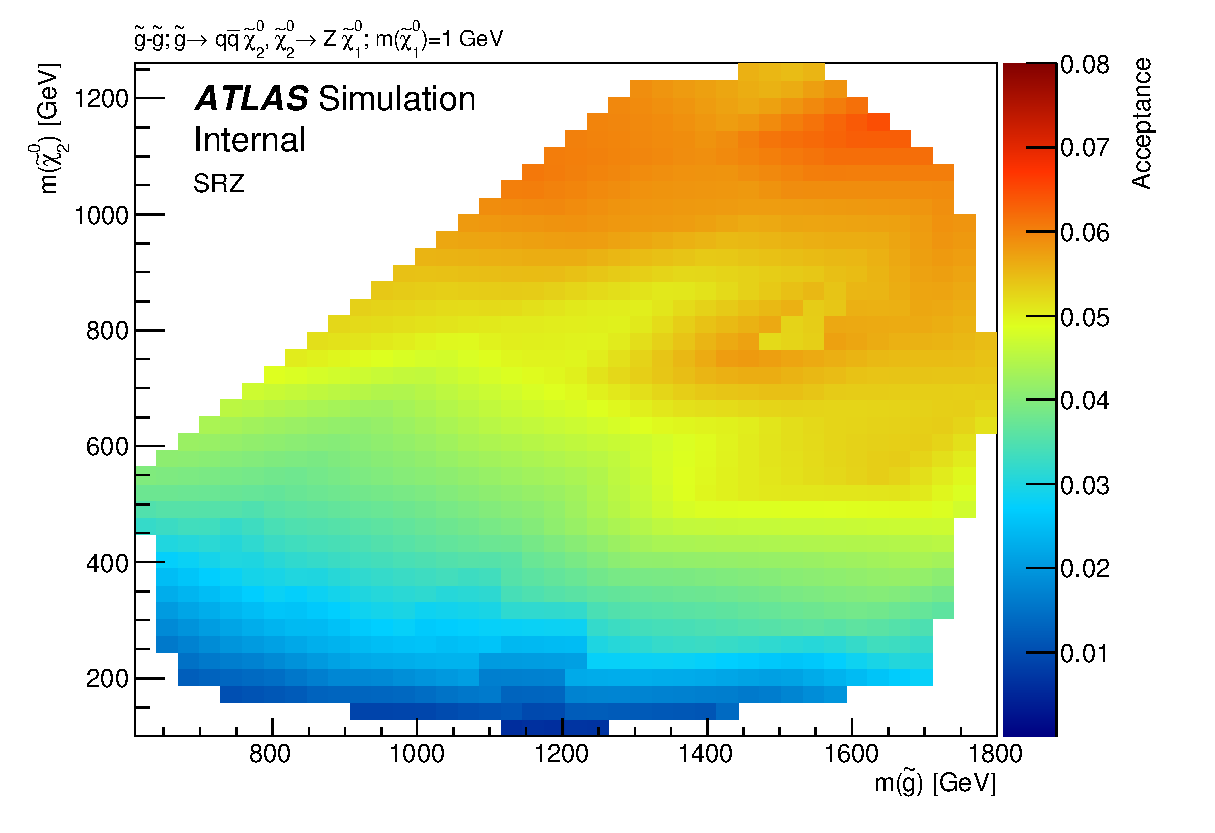
\includegraphics[width=.48\textwidth]{figures/signalacceptcontam/acc_SM_GG_N2_1.eps}
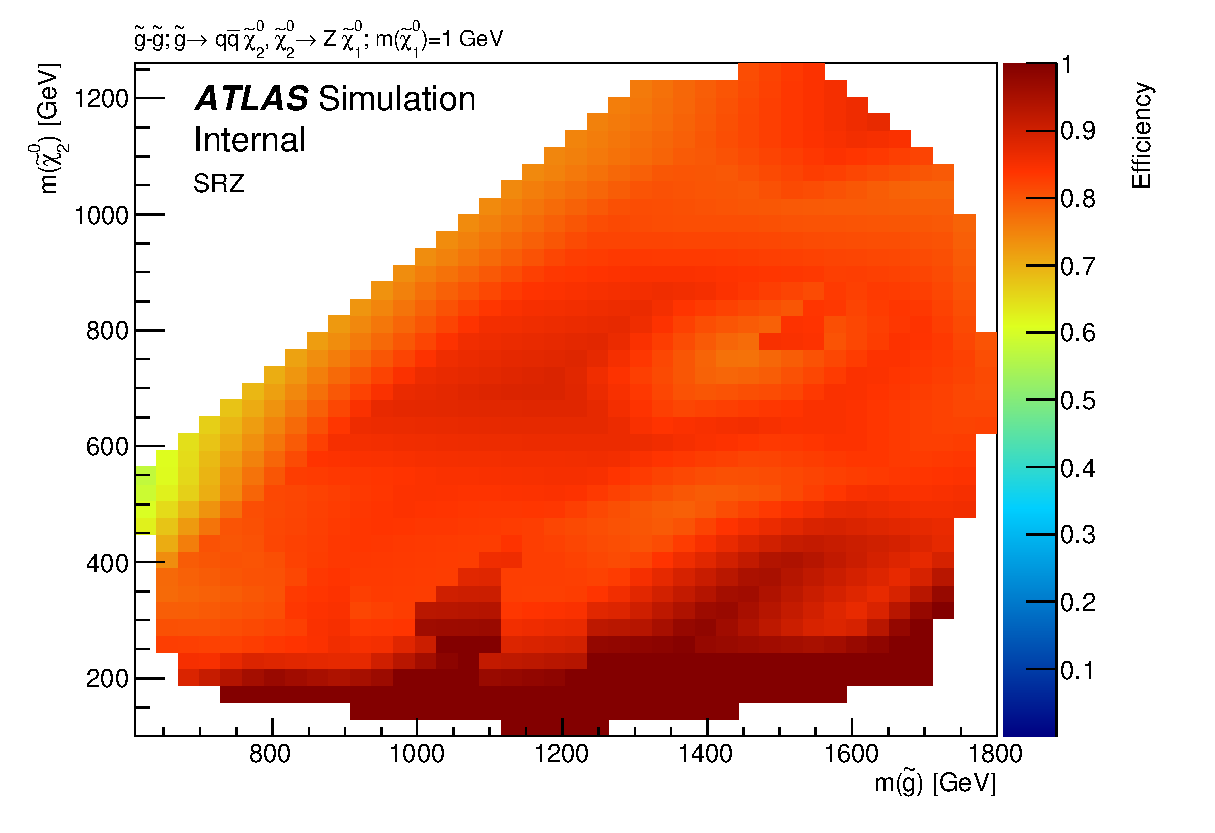
\includegraphics[width=.48\textwidth]{figures/signalacceptcontam/eff_SM_GG_N2_1.eps}
\caption{
Signal region acceptance (left) and efficiency (right) in SRZ for the simplified model with gluino pair production with \chitwozero\ decays to \chionezero and an on-shell $Z$ boson with 1 \gev~neutralino LSP.  
Acceptance is calculated by applying the signal-region kinematic requirements to truth objects in \ac{MC}, which do not suffer from identification inefficiencies or measurement resolutions \cite{this_paper}.
}
\label{fig:acc_SMGGN2_1_z}
\end{figure}

Using the same \ac{MC}, the possibility of signal contamination in the \acp{CR} and \acp{VR} is assessed. Figures~\ref{fig:sig_contam_CRT} and~\ref{fig:sig_contam_VR} show the fraction of events in these regions expected to come from signal for different points on the simplified model's mass grid. Contamination is highest in VRS, at low $m_\go$. However, past analyses have already excluded most models with $m_\go < 800 \gev$ \cite{SUSY-2014-10}, so this is not a concern. For models with $m_\go$ > 800 \gev, signal contamination in VRS is below 30\%, and for models with $m_\go$ > 1 \tev, the contamination decreases to 10\%. In the \acp{CR}, contamination is below 20\% for models with $m_\go$ > 800 \gev, and below 5\% for models with $m_\go$ > 1 \tev. 

\begin{figure}[ht]
\centering
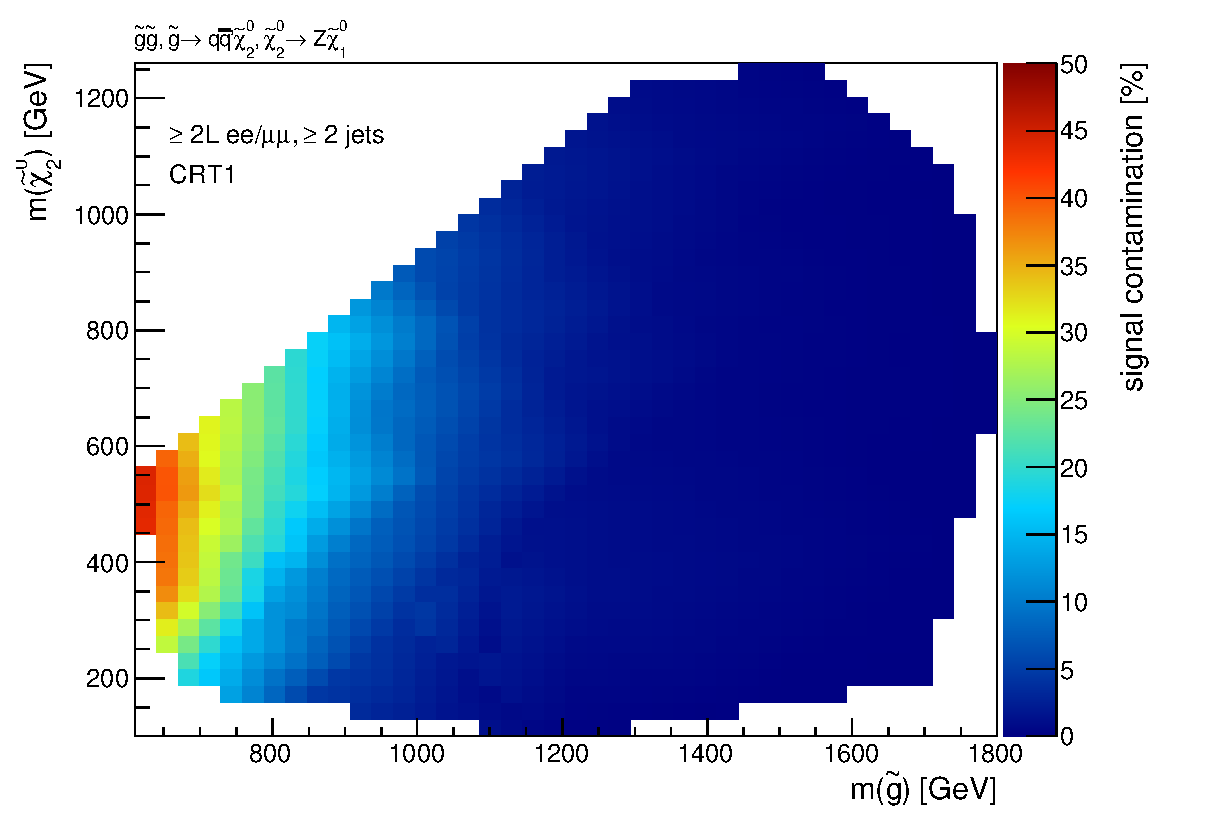
\includegraphics[width=.48\textwidth]{figures/signalacceptcontam/cont_SM_GG_N2_1_CRT1.eps}
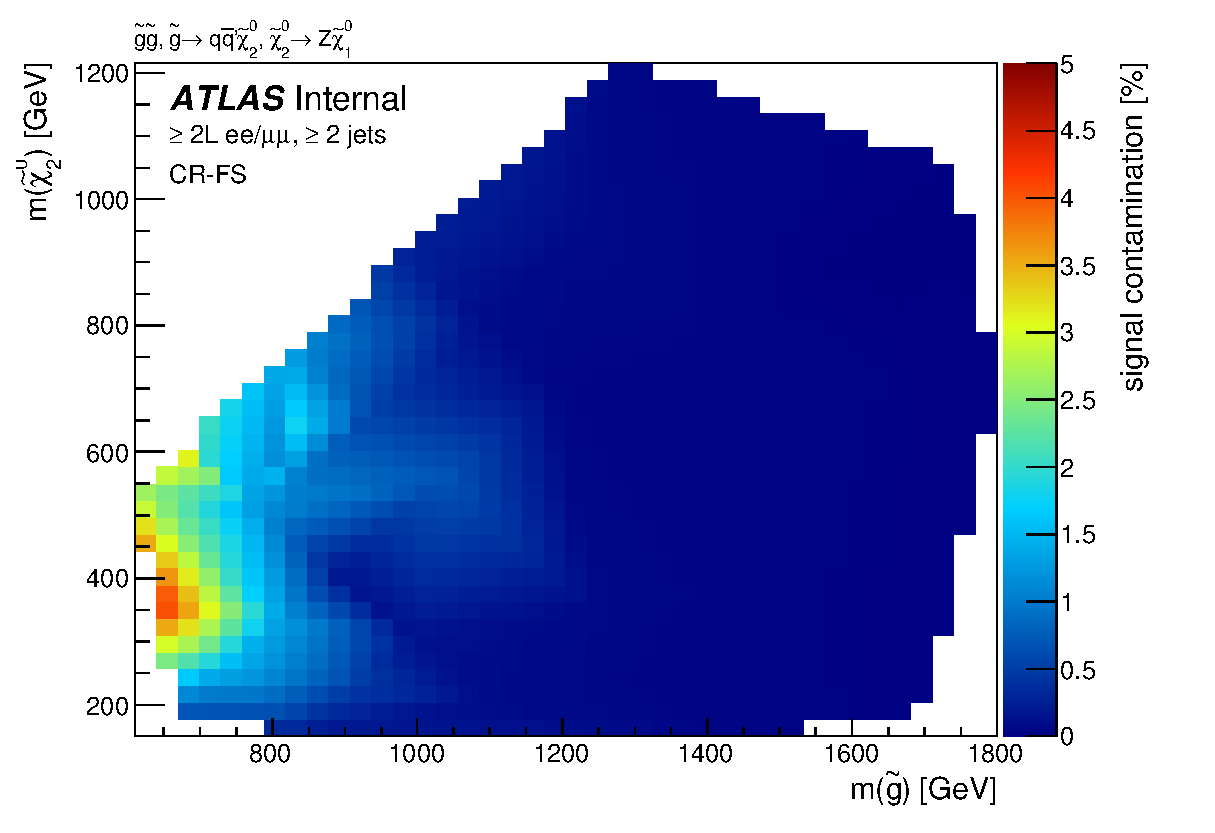
\includegraphics[width=.48\textwidth]{figures/signalacceptcontam/cont_SM_GG_N2_1_CR-FS.eps}
\caption{
Expected signal contamination in CRT (left) and CR-FS (right) for the signal model with gluino pair production, where the gluinos decay to quarks and a neutralino, 
with the neutralino subsequently decaying to a $Z$ boson and a 1 \gev~neutralino LSP.}
\label{fig:sig_contam_CRT}
\end{figure}

\begin{figure}[ht]
\centering
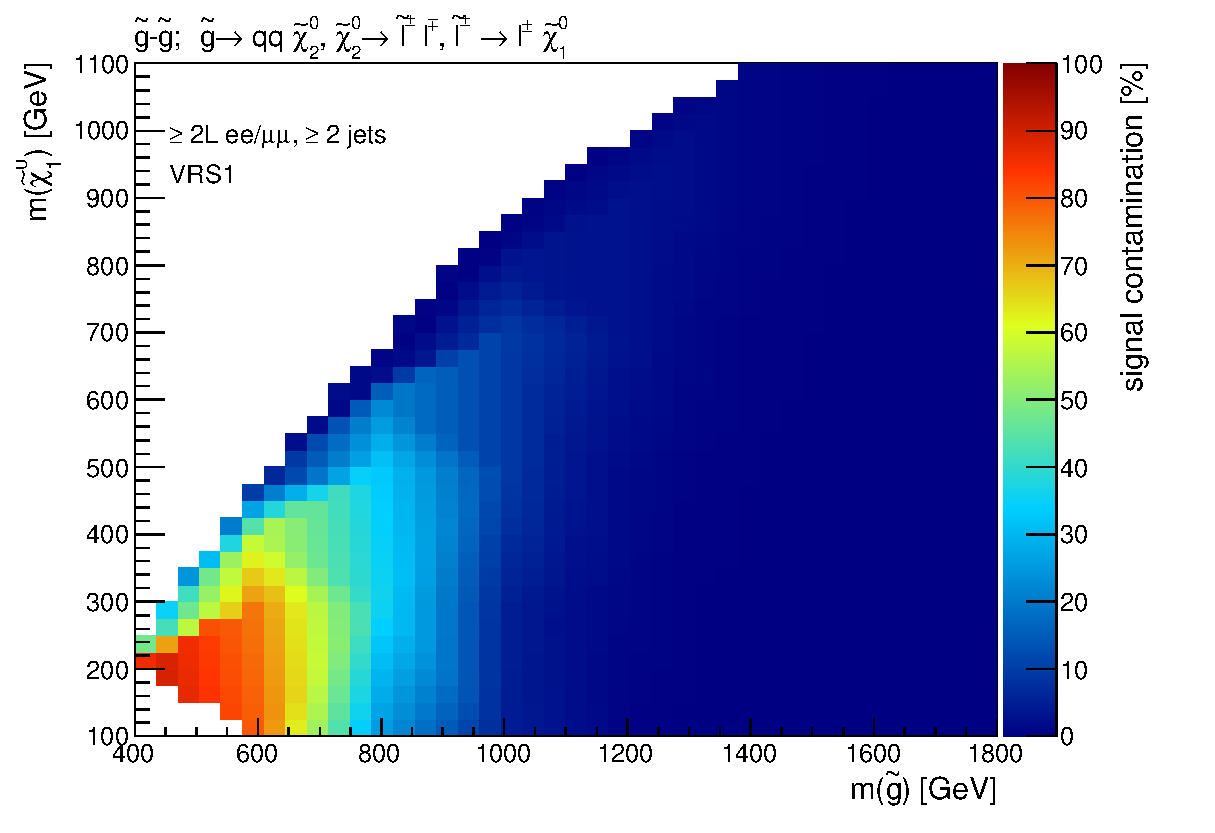
\includegraphics[width=.48\textwidth]{figures/signalacceptcontam/cont_SM_GG_N2_1_VRS1.eps}
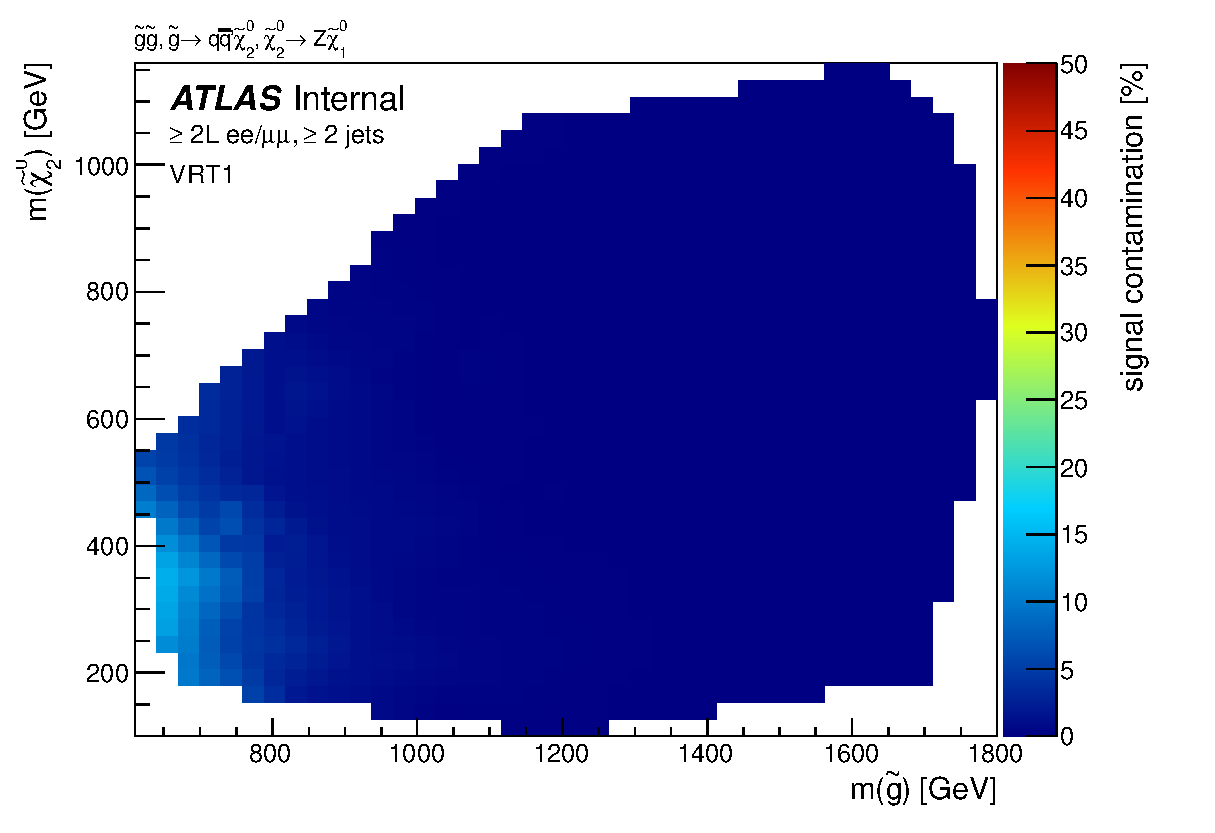
\includegraphics[width=.48\textwidth]{figures/signalacceptcontam/cont_SM_GG_N2_1_VRT1.eps}
\caption{
Expected signal contamination in VRS (left) and VRT (right) for the signal model with gluino pair production, where the gluinos decay to quarks and a neutralino, 
with the neutralino subsequently decaying to a $Z$ boson and a 1 \gev~neutralino LSP.}
\label{fig:sig_contam_VR}
\end{figure}

